\section{Language Evolution}

The previous sections have shown how to build a language extension for mbeddr in
\ac{MPS}, define a debugger for this extension and use \ic{DeTeL} to test its
debugging behavior.
This section demonstrates how \ic{DeTeL} is used to locate invalid definitions
in debugger extensions after evolving the language.

\subsection{Evolving MUnit}

In this section we modify the MUnit generator to reduce the amount of C
code that it generates. Currently, the generator reduces an
\ic{ExecuteTestExpression} to a \ic{FunctionCall} that calls a helper
\ic{Function}, which then calls the reduced \ic{Testcase}s (see \lst{lst:generatedUT}).
We modify this generator, so \ic{ExecuteTestExpression} is reduced to
\ic{FunctionCall}s, which directly call the reduced \ic{Testcase}. In case of
referencing more than one \ic{Testcase}, the \ic{FunctionCall}s are concatenated
via \ic{PlusExpression}s to return the overall number of failed
\ic{Testcase}s. The listing below shows for the \emph{main} \ic{Function}
from \lst{lst:generatedUT} how our generator change affects the generated code. 

\vspace{-2mm}
\noindent 
\hspace{1.2mm}
\begin{minipage}[t]{120pt} 
\begin{lstlisting}[language=reducedMbeddr,numbers=left]
int32 main(int32 argc,
		string[] argv) {
   return $\colorbox{g1}{test[}$$\colorbox{g6}{forTest}$$\colorbox{g1}{]}$;
}
\end{lstlisting}
\end{minipage} 
\rule[-10ex]{0.1ex}{4.0em}
\hspace{0.75mm}
\begin{minipage}[t]{125pt} 
\begin{lstlisting}[language=reducedMbeddr,numbers=left]
int32_t main(int32_t argc,
		char *(argv[])) {
   return $\colorbox{g6}{test\_forTest()}$;
}  
\end{lstlisting}
\end{minipage} 
\vspace{-4mm}
\begin{lstlisting}[caption={Parts of the example program
from \lst{lst:generatedUT} using \emph{MUnit} on the left and the C code
generated from it with our modified generator},
language=mbeddr,label=lst:newGeneratedUT]
\end{lstlisting}


Because of our generator modification, \ic{ExecuteTestEx- pression} is not
reduced to a \ic{Function}, but to an \ic{Expression}. However, we have not
updated the debugger extension, therefore, the call stack construction for all test cases
will fail and this way the tests will fail as well. Although those debugger
tests fail, they are still valid, because they are written on the abstraction level of
the languages, not the generator. The next section shows how we update the
debugger extension to solve the call stack construction problem.

\begin{figure}[h]
	\vspace{-2mm}
	\centering
    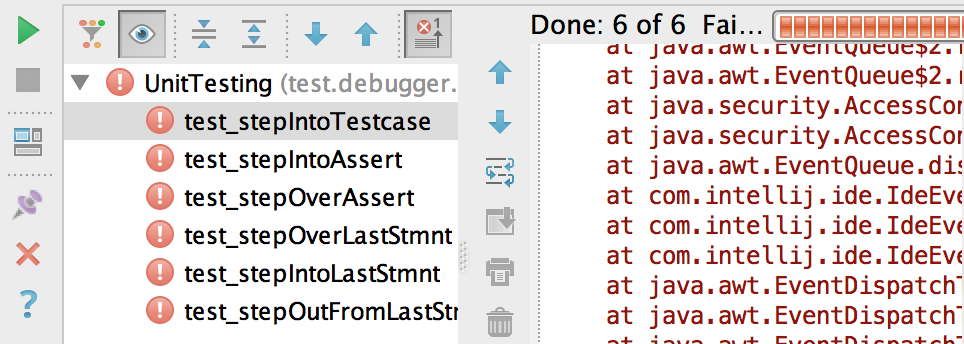
\includegraphics[width=8.5cm]{./figures/failingDebuggerTests.png} 
    \vspace{-3mm}
	\caption{Failing \ic{DebuggerTestcase}s after modifying the generator}
	\label{fig:TestExecution2}
	\vspace{-2mm}
\end{figure}

\subsection{Updating the Debugger Extension}

Because \ic{ExecuteTestExpression} is generated to an \ic{Expression} containing
calls to the referenced \ic{Testcase}s, our call stack lifting is now wrong.
This lifting expects to contribute a \ic{StackFrame} for the generated
\ic{Function}, which is not generated anymore.
To solve the problem, we remove the implementation of \ic{StackFrameContributor} from
\ic{ExecuteTestExpression}. Other aspects such as stepping, breakpoints
and watches are not affected by the generator modification and hence do not need
to be changed. After removing the interface implementation, all of our debugger
tests pass again.